\documentclass[11pt]{article}
\usepackage[margin=1in]{geometry}
\usepackage{amsmath,amssymb,amsthm,mathtools}
\usepackage{booktabs}
\usepackage{graphicx}
\usepackage{tikz}
\usetikzlibrary{arrows.meta,positioning,backgrounds}
\usepackage{hyperref}
\usepackage{longtable}
\usepackage{array}
\newtheorem{theorem}{Theorem}
\newtheorem{lemma}[theorem]{Lemma}
\newtheorem{proposition}[theorem]{Proposition}
\newtheorem{corollary}[theorem]{Corollary}
\newtheorem{definition}[theorem]{Definition}
\newtheorem{remark}[theorem]{Remark}
\newenvironment{sourceresult}[1]{\par\medskip\noindent\textbf{#1.}\ \itshape}{\par\medskip}
\sloppy
\emergencystretch=3em

\title{Formal Verification Report: Theorem 1.1}
\author{Black Swan Labs FCVE \\ ledger through EVENT-014}
\date{2026-09-19}
\begin{document}
\maketitle

\noindent\textbf{Trust Statement.} The formal result was checked using Lean 4.28.0 under the pinned project environment (Mathlib v4.28.0 pin). The theorem CLAIM-001 was kernel-checked with axiom footprint propext, Classical.choice, Quot.sound. Independent checking status is CHECKER\_INCOMPATIBLE for results\_eliahou\_theorem\_1\_1 specifically (no verdict: the external checker could not process this proof's export). Computational/adversarial testing produced: COMPUTATIONALLY\_SUPPORTED (diagnostic only). The remaining trust limitations are: The independent check (Gate 9) produced no verdict; The report (Gate 12) was not recorded; The proof uses Classical.choice; it is a classical proof; The repository, commit and toolchain were captured after the run (on 2026-09-19), not recorded during it; they describe the project as it is now, and the commit matches the one named in the run's own notes; The checker used for the independent check is not identified in the record; only its result is; The recorded result of EVENT-006 refers to a log or receipt that is not part of this report (``see prior receipt for full log''), so that material cannot be inspected here; No counterexample was sought against the underlying nontrivial-cycle claim; that is infeasible. This report does not claim that computational testing constitutes formal proof or that formalization alone establishes the truth of the original informal statement.

\begin{abstract}
This report documents the formal verification of Theorem 1.1 (CLAIM-001) under the Formal Claim Verification Engine. Recorded: build PASS (8033/8033 jobs; see prior receipt for full log); axiom footprint propext, Classical.choice, Quot.sound; independent check CHECKER\_INCOMPATIBLE for results\_eliahou\_theorem\_1\_1 specifically (no verdict: the external checker could not process this proof's export). Computational testing is diagnostic and is not proof. Section 17 states the status the recorded evidence permits; the governance decision is recorded separately, after this report.
\end{abstract}

\section{Mathematical Statement}
\begin{sourceresult}{Theorem 1.1}
Let \ensuremath{\Omega} be a nontrivial cycle of T. Provided min \ensuremath{\Omega} > 2\textasciicircum{}40, we have Card \ensuremath{\Omega} = 301994a + 17087915b + 85137581c, where a,b,c are nonnegative integers, b>0, and ac=0. In particular, the smallest admissible values for Card \ensuremath{\Omega} are 17087915, 17389909, 17691903, and so on.
\end{sourceresult}
Source location: eliahou-collatz.pdf, pages 46, 55-56.

\noindent Facts the statement relies on:
\begin{itemize}
\item p\_13 = 301994, q\_13 = 190537 (Table 1, n=13)
\item p\_15 = 17087915, q\_15 = 10781274 (Table 1, n=15)
\item p\_16 = 85137581, q\_16 = 53715833 (Table 1, n=16)
\item K(2\textasciicircum{}39) = p\_13 = 301994 (p.55: the transition point tr(13,0) is near 2\textasciicircum{}39)
\item K(2\textasciicircum{}40) = K(2\textasciicircum{}48) = p\_15 = 17087915 (p.55: the next transition point tr(15,0) is near 2\textasciicircum{}48)
\item p\_16/q\_16 < log2(3) < p\_15/q\_15 < log2(3+2\textasciicircum{}-40) < p\_13/q\_13 (p.55, from Tables 1-2)
\end{itemize}
\section{Definitions and Assumptions}
\subsection*{Definitions}
\begin{itemize}
\item T: N -> N, T(n) = n/2 if n even, (3n+1)/2 if n odd (p.45)
\item trajectory: Omega(n) = \{n, T(n), T\textasciicircum{}(2)(n), ...\} (p.45)
\item cycle of length k: a trajectory Omega with T\textasciicircum{}(k)(x)=x for all x in Omega, where k = Card Omega (p.45) -- 'length k' is DEFINED to equal Card Omega, not merely correlated with it
\item trivial cycle: Omega(1) = \{1,2\}, the only cycle containing 1 under the 3x+1 conjecture (p.45)
\item theta = log2(3), an irrational number; [a0,a1,a2,...] its continued fraction expansion (p.50)
\item p\_n/q\_n: the principal convergents to theta, defined recursively by p\_n=a\_n*p\_\{n-1\}+p\_\{n-2\}, q\_n=a\_n*q\_\{n-1\}+q\_\{n-2\} (p.51, eq 3.2)
\item Farey pair: (p/q),(p'/q') with pq'-p'q=+-1 (p.49)
\item K(m): the smallest positive integer k such that log2(3) < k/l <= log2(3+1/m) for some positive integer l (p.48, p.52)
\end{itemize}
\begin{remark}\textit{Not recorded: assumptions.json.} This input was not captured during the run, so nothing is shown in its place.\end{remark}
\section{Proof Outline}
\begin{enumerate}
\item \textbf{step 1.} Corollary 2.3 (via Theorem 2.1 + definition of K,L): Card Omega >= K(min Omega), Card Omega1 >= L(min Omega)
\item \textbf{step 2.} Set k = Card Omega, l = Card Omega1. By Theorem 2.1, log2(3+M\textasciicircum{}-1) < k/l <= log2(3+m\textasciicircum{}-1); since M >= m > 2\textasciicircum{}40, k/l lies in the open interval (log2(3), log2(3+2\textasciicircum{}-40))
\item \textbf{step 3.} That interval sits strictly between three specific convergents: p\_16/q\_16 < log2(3) < p\_15/q\_15 < log2(3+2\textasciicircum{}-40) < p\_13/q\_13
\item \textbf{step 4 case split.} k/l falls into exactly one of three regions, each handled by Lemma 3.1 (Farey-pair intermediate-fraction structure): (i) k/l in (p\_16/q\_16, p\_15/q\_15) => k = p\_15*b + p\_16*c for some b,c in N; (ii) k/l = p\_15/q\_15 exactly => k = p\_15*b for some b in N; (iii) k/l in (p\_15/q\_15, p\_13/q\_13) => k = p\_13*a + p\_15*b for some a,b in N
\item \textbf{step 5.} Since the three cases are mutually exclusive and each includes a nonzero p\_15 (=17087915) term, combining them gives Card Omega = 301994a + 17087915b + 85137581c with b>0 always, and a*c=0 because no single case ever produces both a nonzero a AND a nonzero c simultaneously
\end{enumerate}
\begin{sourceresult}{Lemma 2.2}
Let Omega, Omega1 be as above, and let k = Card Omega. Then prod\_\{n in Omega1\} (3+n\textasciicircum{}-1) = 2\textasciicircum{}k.
\end{sourceresult}
\begin{sourceresult}{Theorem 2.1}
Let Omega be a cycle of T, and let Omega1 subset Omega denote the subset of its odd elements. Then log2(3+M\textasciicircum{}-1) < Card(Omega)/Card(Omega1) <= log2(3+m\textasciicircum{}-1), where M=max Omega, m=min Omega. In fact, a sharper right inequality holds: Card(Omega)/Card(Omega1) <= log2(3+mu), where mu = (1/Card Omega1) * sum\_\{n in Omega1\} n\textasciicircum{}-1.
\end{sourceresult}
\begin{sourceresult}{Lemma 3.1}
Let p/q < p'/q' be a Farey pair. Then any intermediate fraction p/q < x/y < p'/q' with y>0 is of the form x/y = (ap+bp')/(aq+bq') where a,b are positive integers. In particular, x >= p+p' and y >= q+q'.
\end{sourceresult}
\begin{sourceresult}{Corollary 2.3}
Let Omega be a cycle of T, and let Omega1 subset Omega denote the subset of its odd elements. Then Card Omega >= K(min Omega), Card Omega1 >= L(min Omega).
\end{sourceresult}
\begin{sourceresult}{Theorem 3.2}
Let theta > 0 be irrational, theta' any number with theta < theta' < [theta]+1. If k,l are positive integers with theta < k/l <= theta', and either k or l is minimal for this property, then k/l is one of the upper convergents to theta -- precisely, the largest upper convergent <= theta'.
\end{sourceresult}
\section{Proof Dependency Diagram}
\begin{center}
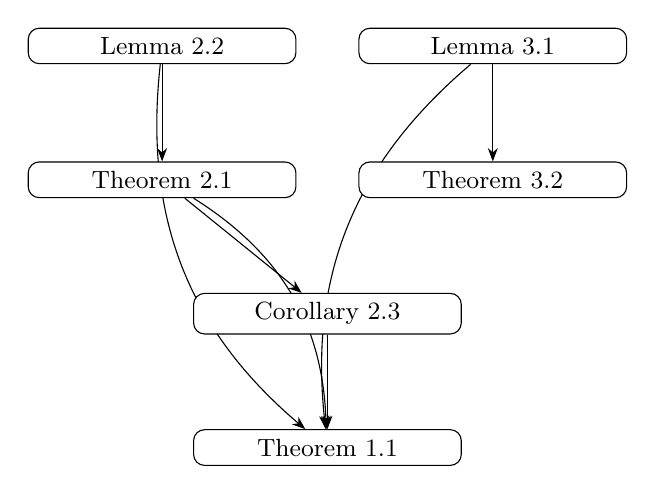
\begin{tikzpicture}[box/.style={draw,rounded corners,align=center,minimum width=34mm,font=\small,fill=white}, >=Stealth]
\node[box] (LEMMA001) at (-2.1,0.0) {Lemma 2.2};
\node[box] (LEMMA003) at (2.1,0.0) {Lemma 3.1};
\node[box] (LEMMA002) at (-2.1,-1.7) {Theorem 2.1};
\node[box] (LEMMA005) at (2.1,-1.7) {Theorem 3.2};
\node[box] (LEMMA004) at (0.0,-3.4) {Corollary 2.3};
\node[box] (CLAIM001) at (0.0,-5.1) {Theorem 1.1};
\begin{scope}[on background layer]
\draw[->, bend right=28] (LEMMA001) to (CLAIM001);
\draw[->, bend left=28] (LEMMA002) to (CLAIM001);
\draw[->, bend right=28] (LEMMA003) to (CLAIM001);
\draw[->] (LEMMA004) to (CLAIM001);
\draw[->] (LEMMA001) to (LEMMA002);
\draw[->] (LEMMA002) to (LEMMA004);
\draw[->] (LEMMA003) to (LEMMA005);
\end{scope}
\end{tikzpicture}
\end{center}
\section{Formalization}
Lean identifiers below are cross-references; the mathematics is in the sections above (\S{}29).
\subsection*{results\_eliahou\_theorem\_1\_1}
{\footnotesize\ttfamily\raggedright\hangindent=1.4em\hangafter=1\noindent
\hspace*{0.00em}theorem results\_\allowbreak{}eliahou\_\allowbreak{}theorem\_\allowbreak{}1\_\allowbreak{}1 \{L : \ensuremath{\mathbb{N}}\} (c : CollatzCycle L)\par
\hspace*{2.20em}(hinj : Function.\allowbreak{}Injective c.\allowbreak{}seq)\par
\hspace*{2.20em}(hmin : (2 : \ensuremath{\mathbb{N}}) \textasciicircum{} 40 < c.\allowbreak{}minElem) :\par
\hspace*{2.20em}\ensuremath{\exists} (a b cCoeff : \ensuremath{\mathbb{N}}), 0 < b \ensuremath{\wedge} a * cCoeff = 0 \ensuremath{\wedge}\par
\hspace*{3.30em}(Finset.\allowbreak{}univ.\allowbreak{}image c.\allowbreak{}seq).\allowbreak{}card =\par
\hspace*{4.40em}301994 * a + 17087915 * b + 85137581 * cCoeff\par
}

\section{Semantic Bridge}
\subsection*{Informal Statement}
Let \ensuremath{\Omega} be a nontrivial cycle of T. Provided min \ensuremath{\Omega} > 2\textasciicircum{}40, we have Card \ensuremath{\Omega} = 301994a + 17087915b + 85137581c, where a,b,c are nonnegative integers, b>0, and ac=0. In particular, the smallest admissible values for Card \ensuremath{\Omega} are 17087915, 17389909, 17691903, and so on.
\subsection*{Normalized Statement}
\begin{remark}\textit{Not recorded: normalized claim file.} This input was not captured during the run, so nothing is shown in its place.\end{remark}
\subsection*{Lean Statement}
{\footnotesize\ttfamily\raggedright\hangindent=1.4em\hangafter=1\noindent
\hspace*{0.00em}theorem results\_\allowbreak{}eliahou\_\allowbreak{}theorem\_\allowbreak{}1\_\allowbreak{}1 \{L : \ensuremath{\mathbb{N}}\} (c : CollatzCycle L)\par
\hspace*{2.20em}(hinj : Function.\allowbreak{}Injective c.\allowbreak{}seq)\par
\hspace*{2.20em}(hmin : (2 : \ensuremath{\mathbb{N}}) \textasciicircum{} 40 < c.\allowbreak{}minElem) :\par
\hspace*{2.20em}\ensuremath{\exists} (a b cCoeff : \ensuremath{\mathbb{N}}), 0 < b \ensuremath{\wedge} a * cCoeff = 0 \ensuremath{\wedge}\par
\hspace*{3.30em}(Finset.\allowbreak{}univ.\allowbreak{}image c.\allowbreak{}seq).\allowbreak{}card =\par
\hspace*{4.40em}301994 * a + 17087915 * b + 85137581 * cCoeff\par
}

\subsection*{Differences}
\begin{remark}\textit{Not recorded: Gate 4 comparison.} This input was not captured during the run, so nothing is shown in its place.\end{remark}
Syntactic signals in the Lean statement that a reviewer must address: injectivity ['Function.Injective'], finite\_structure ['.card', 'Finset'], strictness ['<'].
\subsection*{Findings recorded by the reviewer}
\begin{itemize}
\item \textbf{added hypotheses} (disclosed): hinj : Function.Injective cyc.seq is an extra hypothesis of the Lean theorem that the paper does not state (Gate 4: 'Extra hypothesis'); it is the encoding hypothesis, see Section 31 disclosure.
\item \textbf{coercions} (disclosed): The proof passes through R/Q intermediate steps (rat\_of\_real\_div\_lt) that the paper does not need; this is in the proof, not in the headline statement, and Gate 4 records it as a formalization convenience because the convergents are already rational.
\item \textbf{injectivity assumptions} (disclosed): hinj : Function.Injective cyc.seq. The paper defines cycle length k as Card Omega (p.45); Lean's CollatzCycle L is an L-indexed sequence that may repeat elements, so injectivity is required to identify L with Card Omega.
\item \textbf{classical assumptions} (disclosed): Classical.choice is in the axiom footprint (Gate 6). The Gate 7 note attributes it to ordinary real-number order decidability (Real.logb, lt\_trichotomy), as in any Mathlib real-analysis argument.
\end{itemize}
\subsection*{Justification}
Gate 4 records MATCH with one structural difference, injectivity: the injectivity hypothesis exactly closes the gap between Lean's more general indexed structure and the paper's definition, so the theorem is neither weakened nor strengthened relative to the paper. The proof also implements the paper's own three-case Farey-pair argument. The remaining disclosed items are the R/Q intermediate steps in the proof and Classical.choice in the footprint.


\subsection*{Representational difference (Section 31)}
\begin{description}
\item[What the object means informally.] Omega is a set of distinct positive integers forming a cycle of the compressed Collatz map T, and the paper defines the cycle's length k to equal Card Omega (p.45).
\item[What Lean's type represents.] cyc : CollatzCycle L, an L-indexed sequence cyc.seq (period L, repetitions allowed); Omega is the Finset (Finset.univ.image cyc.seq) and Card Omega is its .card.
\item[Why the encoding is valid.] With hinj : Function.Injective cyc.seq the indexing is exactly Lean's ExactCollatzCycle (injective indexing), which is what a paper 'cycle' inherently is; Gate 4 notes this was confirmed independently.
\item[Where the property is preserved.] Card Omega is the .card of the image finset in the conclusion; injectivity is what makes that image's size equal the period L.
\item[Whether the equality is literal or transported through an equivalence.] Literal on the image finset: the conclusion states an equality of natural numbers about (Finset.univ.image cyc.seq).card. The step from the paper's set Omega to the indexed sequence is the representational choice, not a transport through an equivalence.
\item[Assumptions that make the translation valid.] hinj (injective indexing) as an explicit theorem hypothesis, and hmin : 2\textasciicircum{}40 < cyc.minElem for the paper's minimum condition.
\end{description}
\subsection*{Verdict}
\noindent\textbf{FAITHFUL WITH EXPLICIT REPRESENTATIONAL DIFFERENCE}\par Set by Wilson. Recorded context: Gate 4 recorded MATCH; Gate 7 recorded PASS -- no undisclosed semantic change; Lean proves numOdd\_pos rather than assuming it (stricter than paper).
\section{Lean Environment}
\begin{tabular}{@{}ll@{}}
\toprule
Lean Version & 4.28.0 \\
Mathlib Version & v4.28.0 pin \\
\bottomrule
\end{tabular}
\section{Formal Verification}
PASS (8033/8033 jobs; see prior receipt for full log).
Source of this field: ledger:EVENT-006.
\section{Axiom Audit}
Actual axiom footprint: propext, Classical.choice, Quot.sound.
Source: parsed-legacy-text:EVENT-007.
Classical.choice is present: the proof is classical, which is reported here and does not by itself fail the audit (\S{}14).
\section{Independent Check}
CHECKER\_INCOMPATIBLE for results\_eliahou\_theorem\_1\_1 specifically -- lean4export stalls on this theorem's large proof closure (reproducible, root-caused: memoization cache reset on every call in Export.lean, not a resource issue). 5 of 9 paper-facing theorems (results\_eliahou\_product\_formula, results\_farey\_pair\_bound, results\_eliahou\_product\_formula\_real, results\_eliahou\_sandwich, results\_log2\_three\_lt\_ratio) DID pass independent check cleanly.
Recording the checker and its version does not by itself establish independence (\S{}17).
\section{Computational / Adversarial Tests}
Counterexample search: COMPUTATIONALLY\_SUPPORTED -- all convergents (p13,p15,p16), both Farey identities, and all three boundary inequalities confirmed. Original MISMATCH was a float64 precision artifact in the test script, not a defect in the claim. [diagnostic, not proof]

Computational test: COMPUTATIONALLY\_SUPPORTED -- see EVENT-010 [diagnostic, not proof]

Neither result is formal proof (\S{}16, \S{}18).
\subsection*{What these tests do not establish}
\begin{itemize}
\item They are not proof of the claim (Sections 16 and 18). A search that finds no counterexample is diagnostic evidence only.
\item The tested domain is not recorded for these results, so this report cannot say which cases were examined.
\item No counterexample was sought against the underlying claim about nontrivial Collatz cycles: doing so would require exhibiting an actual nontrivial cycle, which is computationally infeasible and open-problem-adjacent. The computational checks covered numeric and boundary structure only: the convergents p13, p15 and p16, both Farey identities, and the three boundary inequalities. (stated by Wilson)
\end{itemize}
\section{Verification Limitations}
\begin{longtable}{p{0.16\textwidth}p{0.78\textwidth}}
\toprule Item & Limitation \\ \midrule \endhead
1 & The independent check (Gate 9) produced no verdict. Recorded result: CHECKER\_INCOMPATIBLE for results\_eliahou\_theorem\_1\_1 specifically -- lean4export stalls on this theorem's large proof closure (reproducible, root-caused: memoization cache reset on every call in Export.lean, not a resource issue). 5 of 9 paper-facing theorems (results\_eliahou\_product\_formula, results\_farey\_pair\_bound, results\_eliahou\_product\_formula\_real, results\_eliahou\_sandwich, results\_log2\_three\_lt\_ratio) DID pass independent check cleanly. \\
2 & The report (Gate 12) was not recorded. \\
3 & The proof uses Classical.choice; it is a classical proof. \\
4 & The repository, commit and toolchain were captured after the run (on 2026-09-19), not recorded during it; they describe the project as it is now, and the commit matches the one named in the run's own notes. \\
5 & The checker used for the independent check is not identified in the record; only its result is. \\
6 & The recorded result of EVENT-006 refers to a log or receipt that is not part of this report (``see prior receipt for full log''), so that material cannot be inspected here. \\
7 & No counterexample was sought against the underlying claim about nontrivial Collatz cycles: doing so would require exhibiting an actual nontrivial cycle, which is computationally infeasible and open-problem-adjacent. The computational checks covered numeric and boundary structure only: the convergents p13, p15 and p16, both Farey identities, and the three boundary inequalities (stated by Wilson). \\
\midrule \multicolumn{2}{l}{\textit{Record-keeping notes (these do not change what the verification shows)}} \\ \midrule
8 & 12 of 14 ledger events predate the input/output hash fields and carry none. \\
9 & Events EVENT-009 (MISMATCH\_FOUND); EVENT-010, EVENT-012 (COMPUTATIONALLY\_SUPPORTED) used wording outside the Section 16 vocabulary; each is read as diagnostic evidence, not proof. \\
\bottomrule
\end{longtable}
\section{Verification Matrix}
\begin{longtable}{lllll}
\toprule Gate & Ledger action & Event & Status & Satisfied \\ \midrule \endhead
G0 & source intake & EVENT-001 & PASS & yes \\
G1 & claim extraction & EVENT-013 & PASS & yes \\
G2 & assumption extraction & EVENT-003 & PASS & yes \\
G3 & semantic normalization & EVENT-004 & PASS & yes \\
G4 & lean formalization comparison & EVENT-005 & PASS & yes \\
G5 & lean build & EVENT-006 & PASS & yes \\
G6 & axiom audit & EVENT-007 & PASS & yes \\
G7 & semantic re audit & EVENT-008 & PASS & yes \\
G8 & adversarial computational test & EVENT-010 & DIAGNOSTIC & yes \\
G9 & independent check & EVENT-011 & NO\_VERDICT & no \\
G10 & computational check & EVENT-012 & DIAGNOSTIC & yes \\
G11 & evidence graph & EVENT-014 & PASS & yes \\
G12 & report generation & - & MISSING & no \\
ORDER & canonical chain (\S{}2) & - & PASS & yes \\
\bottomrule
\end{longtable}
\section{Trust / Verification Chain}
\begin{center}
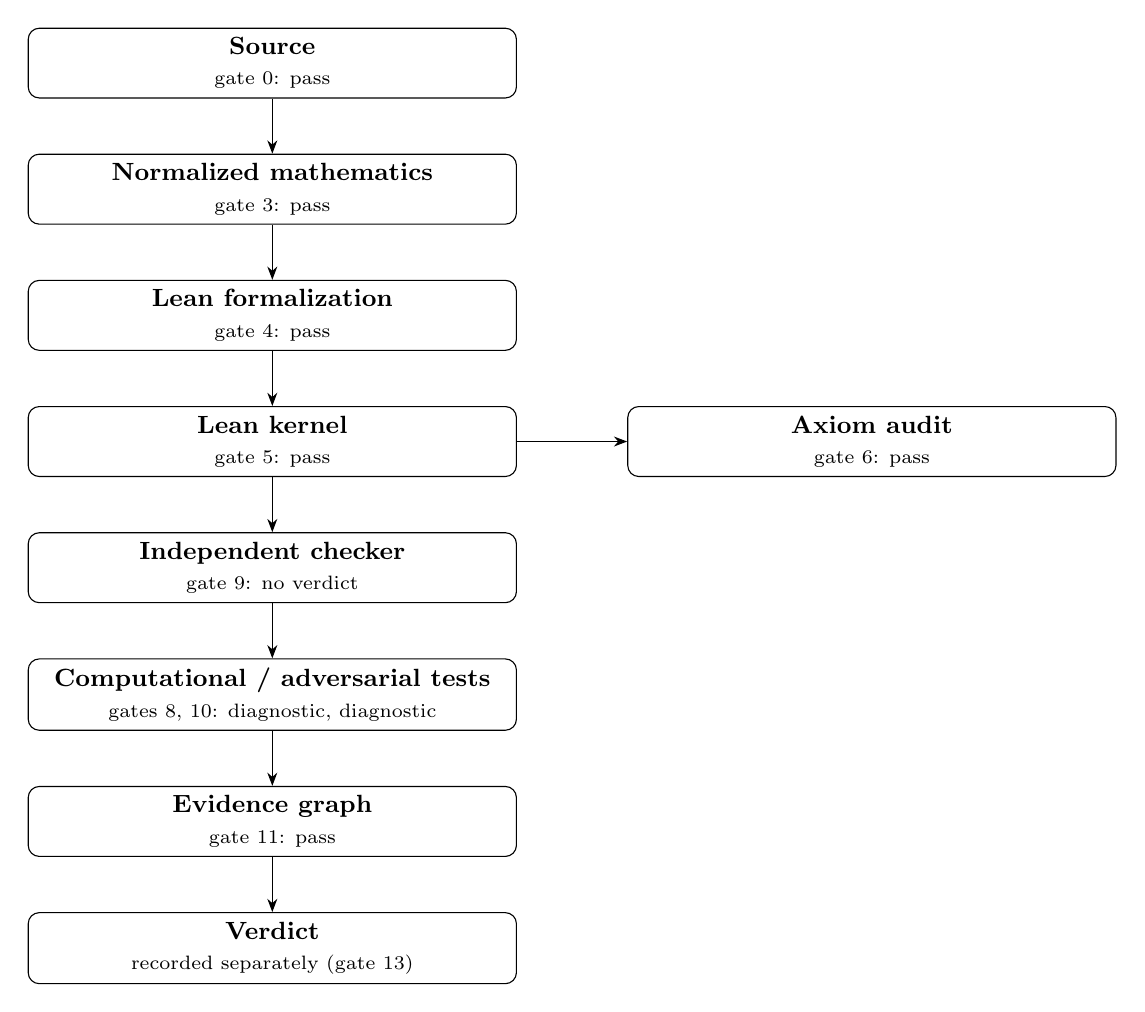
\begin{tikzpicture}[node distance=7mm, box/.style={draw,rounded corners,align=center,minimum width=62mm,font=\small}, >=Stealth]
\node[box] (src) {\textbf{Source}\\{\scriptsize gate 0: pass}};
\node[box, below=of src] (norm) {\textbf{Normalized mathematics}\\{\scriptsize gate 3: pass}};
\draw[->] (src) -- (norm);
\node[box, below=of norm] (lean) {\textbf{Lean formalization}\\{\scriptsize gate 4: pass}};
\draw[->] (norm) -- (lean);
\node[box, below=of lean] (kern) {\textbf{Lean kernel}\\{\scriptsize gate 5: pass}};
\draw[->] (lean) -- (kern);
\node[box, below=of kern] (chk) {\textbf{Independent checker}\\{\scriptsize gate 9: no verdict}};
\draw[->] (kern) -- (chk);
\node[box, below=of chk] (comp) {\textbf{Computational / adversarial tests}\\{\scriptsize gates 8, 10: diagnostic, diagnostic}};
\draw[->] (chk) -- (comp);
\node[box, below=of comp] (evd) {\textbf{Evidence graph}\\{\scriptsize gate 11: pass}};
\draw[->] (comp) -- (evd);
\node[box, below=of evd] (ver) {\textbf{Verdict}\\{\scriptsize recorded separately (gate 13)}};
\draw[->] (evd) -- (ver);
\node[box, right=14mm of kern] (ax) {\textbf{Axiom audit}\\{\scriptsize gate 6: pass}};
\draw[->] (kern) -- (ax);
\end{tikzpicture}
\end{center}
\section{Reproducibility Instructions}
\begin{tabular}{@{}p{0.27\textwidth}p{0.68\textwidth}@{}}
\toprule
Repository URL & https://github\allowbreak{}.com/tangentst\allowbreak{}orm/eliahou-co\allowbreak{}llatz-bounds.g\allowbreak{}it \\
Commit & db804ce6305ea9\allowbreak{}9a817f06786960\allowbreak{}7f8b677d895a (working tree clean) \\
Project directory (now) & /Users/lordwil\allowbreak{}son/ico-collat\allowbreak{}z/targets/elia\allowbreak{}hou-collatz-bo\allowbreak{}unds \\
Lean toolchain file & leanprover/lea\allowbreak{}n4:v4.28.0 \\
Lean version & 4.28.0 \\
Lake version & Lake version 5.0.0-src+7e01\allowbreak{}a1b (Lean version 4.28.0) \\
Mathlib revision & v4.28.0 pin (commit 8f9d9cff6bd728\allowbreak{}b17a24e163c940\allowbreak{}2775d9e6a365) \\
Checker & NOT RECORDED \\
Expected build result & PASS (8033/8033 jobs; see prior receipt for full log) \\
How these were obtained & Captured 2026-09-19 from the project as it is now; not recorded during the run \\
Matches the commit the run's notes name & yes (db804ce6) \\
\bottomrule
\end{tabular}

{\footnotesize\ttfamily\raggedright\hangindent=1.4em\hangafter=1\noindent
\hspace*{0.00em}git clone https:/\allowbreak{}/\allowbreak{}github.\allowbreak{}com/\allowbreak{}tangentstorm/\allowbreak{}eliahou-collatz-bounds.\allowbreak{}git\par
\hspace*{0.00em}cd eliahou-collatz-bounds\par
\hspace*{0.00em}git checkout db804ce6305ea99a817f067869607f8b677d895a\par
\hspace*{0.00em}cat lean-toolchain\par
\hspace*{0.00em}lake --version\par
\hspace*{0.00em}lean --version\par
\hspace*{0.00em}lake exe cache get \&\& lake build\par
\hspace*{0.00em}\# in a Lean file importing the module:  \#print axioms results\_\allowbreak{}eliahou\_\allowbreak{}theorem\_\allowbreak{}1\_\allowbreak{}1\par
\hspace*{0.00em}\# independent-check commands were not recorded for this run\par
}

The repository facts were captured after the run and describe the project as it is now; they do not prove what the original run built. The build command is the one recorded in EVENT-006.
Reproducibility level supported by recorded evidence: R0. This tool did not re-run the build.
\section{Correction Ledger}
\begin{itemize}
\item \textbf{TEST-001} (EVENT-009): MISMATCH\_FOUND (p16/q16 < log2(3) boundary check failed under float64 precision)
\end{itemize}
Gates that produced no verdict (INDEPCHECK-001) are not corrections; they are listed under Verification Limitations.


\section{Conclusion}
The recorded evidence is summarized in the Trust Statement and the verification matrix above. Recorded failure is not a passed gate.
\begin{center}\begin{tabular}{@{}p{0.36\textwidth}p{0.58\textwidth}@{}}
FORMAL PROOF (build): & PASS \\
AXIOM AUDIT: & PASS \\
SEMANTIC MATCH (Gate 4): & PASS \\
SEMANTIC RE-AUDIT (Gate 7): & PASS \\
INDEPENDENT CHECK: & NO VERDICT \\
COUNTEREXAMPLE SEARCH: & NO COUNTEREXAMPLE FOUND IN TESTED DOMAIN (diagnostic, not proof) \\
COMPUTATIONAL TEST: & NO COUNTEREXAMPLE FOUND IN TESTED DOMAIN (diagnostic, not proof) \\
REPRODUCIBILITY: & R0 (ceiling supported by recorded evidence) \\
\end{tabular}\end{center}
%% PERMITTED-STATUS-BEGIN
\begin{quote}\textbf{Status the evidence permits.} Promotion (PROMOTE) is not supported by the recorded evidence, because: G9 (independent check): no verdict. The reviewer may still record REPAIR, REJECT, RESEARCH or STOP. This is not a decision: the governance decision is recorded as a separate step after this report.\end{quote}
%% PERMITTED-STATUS-END
\appendix
\section{Lean Source}
{\footnotesize\ttfamily\raggedright\hangindent=1.4em\hangafter=1\noindent
\hspace*{0.00em}theorem results\_\allowbreak{}eliahou\_\allowbreak{}theorem\_\allowbreak{}1\_\allowbreak{}1 \{L : \ensuremath{\mathbb{N}}\} (c : CollatzCycle L)\par
\hspace*{2.20em}(hinj : Function.\allowbreak{}Injective c.\allowbreak{}seq)\par
\hspace*{2.20em}(hmin : (2 : \ensuremath{\mathbb{N}}) \textasciicircum{} 40 < c.\allowbreak{}minElem) :\par
\hspace*{2.20em}\ensuremath{\exists} (a b cCoeff : \ensuremath{\mathbb{N}}), 0 < b \ensuremath{\wedge} a * cCoeff = 0 \ensuremath{\wedge}\par
\hspace*{3.30em}(Finset.\allowbreak{}univ.\allowbreak{}image c.\allowbreak{}seq).\allowbreak{}card =\par
\hspace*{4.40em}301994 * a + 17087915 * b + 85137581 * cCoeff\par
}

\section{Tests}
\begin{itemize}
\item \textbf{EVENT-009} python3 verification/computational/tests/verify\_convergents.py (initial run, native float boundary comparison): MISMATCH\_FOUND (p16/q16 < log2(3) boundary check failed under float64 precision)
\item \textbf{EVENT-010} python3 verification/computational/tests/verify\_convergents.py (corrected: mpf 60-digit precision for boundary comparisons): COMPUTATIONALLY\_SUPPORTED -- all convergents (p13,p15,p16), both Farey identities, and all three boundary inequalities confirmed. Original MISMATCH was a float64 precision artifact in the test script, not a defect in the claim.
\item \textbf{EVENT-012} Python/mpmath backend (per Section 19 backend abstraction; MATLAB not required): COMPUTATIONALLY\_SUPPORTED -- see EVENT-010
\end{itemize}
\section{Evidence Receipt}
\begin{longtable}{p{0.24\textwidth}p{0.70\textwidth}}
\toprule Field & Value \\ \midrule \endhead
SOURCE HASH & NOT RECORDED \\
THEOREM ID & CLAIM-001 (Theorem 1.1) \\
CLAIM & Let \ensuremath{\Omega} be a nontrivial cycle of T. Provided min \ensuremath{\Omega} > 2\textasciicircum{}40, we have Card \ensuremath{\Omega} = 301994a + 17087915b + 85137581c, where a,b,c are nonnegative integers, b>0, and ac=0. In particular, the smallest admissible values for Card \ensuremath{\Omega} are 17087915, 17389909, 17691903, and so on. \\
NORMALIZED CLAIM & normalized/nor\allowbreak{}malized-claim.\allowbreak{}md -- MATCH \\
LEAN STATEMENT & Gate 4: MATCH \\
LEAN VERSION & 4.28.0 \\
MATHLIB VERSION & v4.28.0 pin \\
BUILD RESULT & PASS (8033/8033 jobs; see prior receipt for full log) \\
AXIOM FOOTPRINT & propext, Classical.choi\allowbreak{}ce, Quot.sound \\
INDEPENDENT CHECK & CHECKER\_INCOMP\allowbreak{}ATIBLE for results\_eliaho\allowbreak{}u\_theorem\_1\_1 specifically -- lean4export stalls on this theorem's large proof closure (reproducible, root-caused: memoization cache reset on every call in Export.lean, not a resource issue). 5 of 9 paper-facing theorems (results\_eliah\allowbreak{}ou\_product\_for\allowbreak{}mula, results\_farey\_\allowbreak{}pair\_bound, results\_eliaho\allowbreak{}u\_product\_form\allowbreak{}ula\_real, results\_eliaho\allowbreak{}u\_sandwich, results\_log2\_t\allowbreak{}hree\_lt\_ratio) DID pass independent check cleanly. \\
COMPUTATIONAL TEST & COMPUTATIONALL\allowbreak{}Y\_SUPPORTED -- see EVENT-010 [diagnostic, not proof] \\
COUNTEREXAMPLE SEARCH & COMPUTATIONALL\allowbreak{}Y\_SUPPORTED -- all convergents (p13,p15,p16), both Farey identities, and all three boundary inequalities confirmed. Original MISMATCH was a float64 precision artifact in the test script, not a defect in the claim. [diagnostic, not proof] \\
SEMANTIC MATCH & Gate 4: MATCH; Gate 7: PASS -- no undisclosed semantic change; Lean proves numOdd\_pos rather than assuming it (stricter than paper) \\
REPRODUCIBILITY LEVEL & R0 (ceiling supported by recorded evidence; NOT re-run by this tool; R5 needs full-package rebuild, not assessed) \\
GRAPH HASH & v3 8558c9b7f7b0e9\allowbreak{}aeb60b0157f026\allowbreak{}864f77d1440d54\allowbreak{}954caa810723ae\allowbreak{}9a62f292 (covers 14 events through EVENT-014) \\
COST & 14 ledger events; LEAN\_BUILD\_TIM\allowbreak{}E=NOT RECORDED; COMPUTATIONAL\_\allowbreak{}TEST\_TIME=NOT RECORDED; CHECKER\_TIME=N\allowbreak{}OT RECORDED; HUMAN\_TIME, MODEL\_CALL\_COU\allowbreak{}NT, MODEL\_COST, LATEX\_BUILD\_TI\allowbreak{}ME=NOT RECORDED (no cost ledger, \S{}43) \\
\bottomrule
\end{longtable}
\end{document}
